%%%%%%%%%%%%%%%%%%%%%%%%%%%%%PREÁMBULO DEL DOCUMENTO%%%%%%%%%%%%%%%%%%%%%%%%%%%
% En esta sección se configura el document, pero no se incluye contenido
% Esto es la clase del documento, que defines las instrucciones principales
% que condicionarán el documento generado. Generalmente cambiarla después de 
% añadir contenido produce numerosos errores.
\documentclass{article}


%%%%%%%%%%%%%%%%%%%SECCIÓN INCLUSIÓN DE PAQUETES %%%%%%%%%%%%%%%%%%%%%%%%%%%%%%
% Este paquete permite cambiar la fuente. Hay muchas, la lista se puede
% encontrar en https://tug.org/FontCatalogue/, las que no indican nada después
% del nombre son las que se pueden usar como está aquí puesto.
\usepackage[T1]{fontenc}
% Comentar esta línea haría que se usara la fuente predeterminada.
\usepackage{newcent}
\usepackage{titlesec}

% Carga el paquete babel, las opciones son:
    % spanish: indica que usaremos configuración para escribir en español
    % es-tabla: traduce la palabra table como tabla, no como cuadro
    % es-lcroman: permite la numeración romanda en minúscula.
\usepackage[spanish, es-tabla, es-lcroman]{babel}
% Paquete que permite escribir el símbolo del euro, se usa de dos maneras.
    % En el documento, la orden \euro escribirá el símbolo
    % Si se escribe \EUR{<cifra>} el paquete formará un bloque con el
    % número y el símbolo.
    % El símbolo del euro que pone es el «oficial» es decir, no se adapta
    % a la fuente que se use.
\usepackage{eurosym} 
% Paquete para que las imágenes tengas un tamaño relativo al del párrafo
\usepackage{graphicx}
% nos permite insertar las figuras con el especificador H, que hace que se
    % inserte en el lugar del document donde se ha escrito su código.
\usepackage{float} 
% Paquete que habilita las referencias cruzadas.
\usepackage{hyperref}
% Permite poner pies y encabezados de página personalizados
\usepackage{fancyhdr}
 %permite referenciar la última página (para incluir páginas totales)
\usepackage{lastpage}
% Paquete BibTex para referencias bibliográficas.
\usepackage[backend=biber, style=alphabetic, sorting=ynt]{biblatex}

% Permite figuras y tablas que sean rodeadas por el texto.
% Este paquete y su funcionalidad dan problemas, no lo recomiendo.
%\usepackage{wrapfig}

\usepackage{geometry}
 \geometry{
    a4paper, % tamaño del papel
    left=30mm, % márgenes laterales
%   top=50mm 
    bottom=35mm, %margen inferior
    headheight=25mm    %margen superior
}
%enables utf8 support
\usepackage[utf8]{inputenc}

%%%%%%%%%%%%%%%%%%%% FIN SECCIÓN %%%%%%%%%%%%%%%%%%%%%%%%%%%%%%%%%%%%%%%%%%%%%%

% Vamos a permitir más niveles de título, hasta 5.
\setcounter{secnumdepth}{5}
% Esto hace que la tabla de contenidos muestre hasta el nivel 3.
    % Si se quiere que la tabla de contenido muestre todos los niveles, sólo
    % ha de cambiarse el 3 por un 5
\setcounter{tocdepth}{3}
% Aquí estamos redefiniendo el comando paragraph, será nuestro título de nivel
    % 4. Esta es una de las cosas que no tengo nada claro cómo funciona, 
    % pero funciona, así que si quieres usar títulos de esta jerarquía, 
    % déjalo así. 
\titleformat{\paragraph}{\bfseries}{\theparagraph .}{1em}{}
\titlespacing*{\paragraph}{0pt}{3.25ex plus 1ex minus .2ex}{1.5ex plus .2ex}

% El subparagraph será el título de nivel 5
\titleformat{\subparagraph}{\bf}{\thesubparagraph .}{1em}{}
\titlespacing*{\subparagraph}{0pt}{3.25ex plus 1ex minus .2ex}{1.5ex plus .2ex}


% Esta línea nos permite indicar un directorio donde estamos guardando
% nuestras imágenes. Más información más adelante.
\graphicspath{{img/}}


% Esto hace que los enlaces a webs (\href{url}{texto} salgan en azul.
    % También impide que salga un repugnante rojo alrededor de cada
    % referencia cruzada que incluyas en el documento.
\hypersetup{
    colorlinks=true,
    linkcolor=black,
    filecolor=magenta,      
    urlcolor=blue,
}
% Permite que en las ecuaciones escribas un punto y salga un punto (no lo
% interprete como un decimal en español, es decir, una coma)
\decimalpoint

% Permite utilizar archivos de fuente bibliográficas
\addbibresource{./bibliography/sources.bib}


%%%%%%%%%%%%%%%%%SECCIÓN VARIABLES %%%%%%%%%%%%%%%%%%%%%%%%%%%%%%%%%%%%%%%%%%%%
% Podemos definir variables para usar a lo largo del texto
% Así podemos cambiarlas aquí sin tener que repetir texto.
\def \autor{Autor Autórez Ejémplez}
\def \titulo{Ejemplo de documento en \LaTeX{}}
\def \organizacion{Universidad de Ejemplo}
%%%%%%%%%FIN SECCIÓN%%%%%%%%%%%%%%%%%%%%%%%%%%%%%%%%%%%%%%%%%%%%%%%%%%%%%%%%%%%

% Esta orden especifica que cuando se cree la portada se use este título.
% Además, con Huge utilizamos la macro de tipo de letra más grande que hay 
% disponible.
\title{\textbf{\Huge{\titulo}}}
% Aquí lo mismo, pero con el autor
% Algunos especificadores de tamaño son: tiny, small, large, Large, LARGE, huge
    % y Huge
\author{\LARGE{\autor}\\ \\ \Large{\organizacion}}
%%%%%%%%%%%%%%%%%%%%%%%%%%%%FIN DEL PREÁMBULO%%%%%%%%%%%%%%%%%%%%%%%%%%%%%%%%%%


%%%%%%%%%%%%%%%%%%%%%%%%%%%%%%INICIO DEL DOCUMENTO%%%%%%%%%%%%%%%%%%%%%%%%%%%%%
% La totalidad del texto que se renderizará en PDF en tu documento debe estar
% entre begin document y end document.
\begin{document}
% Elimina la numeración de página hasta que se diga lo contrario.
\pagenumbering{gobble}
% Pone el título, el autor y la fecha. (la fecha se detecta automáticamente)
\maketitle

% Aquí creamos una figura para poner el logo de algo (Ahora hay un placeholder) 
% más en cuanto a figuras más adelante.
\begin{figure}[H]
    % Lo centramos
    \center
    
\includegraphics[width=.5\linewidth]{escudo}
\end{figure}
\newpage
% En esta página puedes poner agradecimientos o prefacios que no tendrán pie ni
% encabezado de página y que no afectarán a la numeración, si no quieres poner
% nada, elimina esta línea y uno de los newpages
\textbf{[Esta página ha sido dejada en blanco a propósito por el editor]}
\newpage
%Vamos a poner agradecimientos
\begin{flushright}
\textit{Esto es un placeholder, muchas gracias, placeholder.}
\end{flushright}
\newpage % salto de página

%%%%%%%%%%%%%%%%% CABECERA Y PIE DE PÁGINA SECCIÓN ÍNDICE%%%%%%%%%%%%%%%%%%%%%
\pagestyle{fancy}
% Incluye una línea horizontal en el encabezado de página.
\fancyhf{}
% Texto de la parte derecha del encabezado, nótese que usamos la variable
    % que hemos definido anteriormente.
\rhead{\autor}
% Texto de la parte izquierda
\lhead{\titulo}
% Incluye el texto "pág. X de Y" en el pie de pág. a la derecha.
    % estoy referenciando una etiqueta que añadí, se verá luego.
\rfoot{pág. \thepage{} de \pageref{startSectionContent}} 
% Incluye una línea en el pie de página.
\renewcommand{\footrulewidth}{0.5pt}
%decimos que se numeren las páginas en romano hasta nueva orden
    % Esto nos permite numerar las páginas de índices en números romanos
\pagenumbering{roman} 
%%%%%%%%%%%%%%%%%FIN
\tableofcontents %crea el índice el índice empieza siempre en página nueva

% se pueden añadir saltos de página extra con \newpage
\newpage

% cambia el nombre del índice de ilustraciones
\renewcommand{\listfigurename}{Índice de ilustraciones}
%inserta el índice de ilustraciones
\listoffigures 
\newpage

%tambia el nombre del índice de tablas
\renewcommand{\listtablename}{Índice de tablas}

%inserta el índice de tablas
\listoftables

% Esta orden (label) inserta etiquetas invisibles en el texto, al ponerla justo
    % antes del salto de página del último índice de la sección, me permite
    % referenciar este punto, así es como consigo que salga "Pág. i de iiii".
\label{startSectionContent}

\newpage
% A partir de aquí numeración normal
\pagenumbering{arabic}
%%%%%%%%%%%%%%%%% CABECERA Y PIE DE PÁGINA SECCIÓN CUERPO%%%%%%%%%%%%%%%%%%%%%%
\pagestyle{fancy}
\fancyhf{}
\rhead{\autor}
\lhead{\titulo}
% El único cambio es que aquí referencio la última página de verdad.
\rfoot{pág. \thepage{} de \pageref{LastPage}}
\renewcommand{\footrulewidth}{0.5pt}
%%%%%%%%%%%%%%%%%%%%%%%%%%%%%%%%%FIN SECCIÓN%%%%%%%%%%%%%%%%%%%%%%%%%%%%%%%%%%%
% La sección es el primer nivel de título que se permite en esta clase de 
    % documento. Introduce un título de primer nivel
\section{Presentación}
Este documento pretende ser un ejemplo de varias tareas que se suelen realizar
en LaTeX. Se recomienda compilar el código y ver el pdf y el mismo código a la
vez para ver los resultados. En los comentarios del código explico lo que se va
haciendo y qué órdenes son necesarias para crear lo que se ve en el PDF.
Además, incluyo un \textit{script} de compilación mínimo que debería compilar
sin problemas. Los prerrequisitos son:
\begin{itemize}
    \item Sistema operativo GNU/Linux
    \item Herramienta make
    \item Tener \LaTeX{} instalado en el sistema, se puede instalar con la orden
    \begin{verbatim}
$ sudo apt install texlive-base \
                       texlive-latex-recommended \
                       texlive-latex-extra \
                       texlive-full \\end{verbatim} 
En sistemas derivados de Debian. En otras distribuciones, 
por favor, consulte la documentación específica de cómo instalar paquetes de
\textit{software}.
\end{itemize}

Este documento está diseñado para ser una guía básica sobre Latex, pero para
poder generarse, se usarán comandos en el mismo documento antes de explicarlos.
Si se sabe algo sobre \LaTeX{} es recomendable leer el código primero, si no, 
mejor leer primero el pdf compilado. Preveo añadir información sobre ćomo
instalar LaTeX en más plataformas en el futuro.

\section{Qué es exactamente \LaTeX{}}
Aunque en este documento no voy a hablar de las características históricas o de
lo que es el \textit{typesetting}. Sí voy a explicar someramente qué es LaTeX.
LaTeX es un lenguaje que nos permite crear documentos con formato a través de
archivos de texto plano, que no contienen en sí mismos información sobre el
mormato, sino que utilizan secuencias especiales de caracteres para indicar 
cómo ha de presentarse el contenido en un documento distinto.
\subsection{Archivos .tex}
Un archivo .tex es donde escribimos el código -se denomina código al texto
escrito con estos comandos que nos permite luego convertirlos en documentos-
que generará un documento. El
programa que genera el documento (generalmente pdf) a partir del código LaTeX
se llama motor o renderizador. Hay varios, con diferencias técnicas. Esta guía
y los comandos que se listan están desarrollados para el motor 
\texttt{pdflatex}.
\subsubsection{Estructura de un documento en LaTeX}
Un documento en latex mínimo tiene estas líneas:
\begin{verbatim}
\documentclass{<clase del documento>}
\begin{document}
    Algún texto.
\end{document}
\end{verbatim}

La clase del documento será una palabra que definirá un estilo de documento
concreto que nos permita empezar a escribir sin tener que formatearlo todo
desde 0. Las más populares son: article, book y report; pero hay muchas más.
Si se quiere compilar el primer documento en LaTeX, se puede copiar ese código,
pero debe sustituirse \texttt{<clase del documento>} por \texttt{article}.
Este documento se ha escrito con la clase de documento article. Como las clases
de documento definen las instrucciones que se usarán después en el documento,
es muy difícil cambiarla una vez se han escrito y formateado una cuantas
páginas.

Todo lo que hay antes de la línea donde pone 
\texttt{\textbackslash begin\{document\}}, sin incluirla, se denomina el 
preámbulo del documento. Y lo que existe entre la línea
\texttt{\textbackslash begin\{document\}} y la línea
\texttt{\textbackslash end\{document\}} se considera el contenido del
documento. Además, por su herencia o similitud con otros lenguages formales,
de programación y de marcado, \LaTeX{} tiene la posibilidad de incluir 
comentarios en el código. Esto es texto que el renderizador no lee. En \LaTeX{}
dichos comentarios se ponen con el signo de porcentaje <<\%>>. Cualquier
texto en un archivo \texttt{.tex} que vaya en la misma línea que un signo de
procentaje y después de él no se renderizará. \textbf{Esto incluye el salto
de lína del final}. Veamos un ejemplo:
\begin{verbatim}
\documentclass{article}
\begin{document} % Aquí puedo escribir lo que quiera
Algún texto de un párrafo.
% Este exto no va a salir
% Este tampoco.
Otro texto de otro párrafo.
\end{document}
\end{verbatim}

Además de que no se van a renderizar los texto de los comentarios, estos
dos párrafos son uno, porque se eliminan las líneas enteras, así que habría
que poner una línea en blanco entre el último comentario y el segundo
párrafo.

\subsection{Escritura de texto en \LaTeX{}}
Como se ha visto en la sección anterior, dentro del contenido del documento es
donde se puede incluir texto. Ahora bien, si has experimentado con este archivo 
\texttt{.tex}.
que has creado con el código anterior, quizás hayas notado que los saltos de
línea no se trasladan a párrafos distintos.
En Latex, un párrafo es una línea de texto o varias líneas consecutivas, que se
renderizan siempre en el mismo párrafo salvo que haya un salto de línea entre
ellas. Por ejemplo, vamos a poner un punto y aparte. Es decir:
\begin{verbatim}
\documentclass{article}
\begin{document}
Algún texto de un párrafo.

Otro texto de otro párrafo.
\end{document}
\end{verbatim}

Además, \LaTeX{} permite utlizar varios
comandos para manipular la presentación del texto.
\begin{itemize}
    \item \textbf{emph:} Pone el texto en énfasis.
    \item \textbf{textit:} Pone el texto en itálica (o cursiva).
    \item \textbf{textbf:} Pone el texto en negrita. 
    \item \textbf{texttt:} Utiliza fuente monoespaciada (como la de las máquinas
    de escribir).
\end{itemize}
Estos comandos deben ponerse en nuestros archivos \texttt{.tex}
con una barra inclinada hacia atrás delante, como todos los comandos de \LaTeX{}
.
Y seguidos de dos llaves,
dentro de las cuales incluiremos el texto que queramos modificar. Por ejemplo:
\begin{verbatim}
Este es el primer párrafo de esta sección,
en cualquier texto podemos incluir texto en
\textbf{negrita} o en \textit{cursiva}, incluso,
podríamos incluir texto en 
\textbf{\textit{negrita y cursiva}}. 
\end{verbatim}
sería el código en \LaTeX{} que renderizaría el párrafo que se ve a continuación:


% párrafo con texto en distintos formatos, textit es itálita, textbf es 
% negrita, se pueden combinar. texttt es monoespaciada, la uso luego
% Como puedes ver, aunque hay saltos de línea, no son párrafos distintos.
% Para que sean párrafos distintos tiene que haber una línea en blanco
% entre ellos.
Este es el primer párrafo de esta sección, en cualquier texto
podemos incluir texto en
\textbf{negrita} o en \textit{cursiva}, incluso, podríamos incluir texto en 
\textbf{\textit{negrita y cursiva}}.

Si queremos escribir comandos u órdenes
de programación, podemos ponerlo en monoespaciado: \texttt{ls -la}.
Además, el comando de énfasis (\texttt{emph}) nos maneja el énfasis automáticamente.
Por ejemplo, el código:
\begin{verbatim}
\emph{\emph{Toda} esta frase está en énfasis
menos la primera y la última \emph{palabra}}.
\end{verbatim}
Producirá el siguiente párrafo:

<<\emph{\emph{Toda} esta frase está en énfasis
menos la primera y la última \emph{palabra}}.>>
Esto es porque la orden emph, cuando se aplica a un texto enfatizado, elimina
la letra itálica, como es la norma.

Además de texto, es natural que en un 
documento tengamos que poner listas, ya sean éstas numeradas o sin numerar.
A continuación vemos cómo se hace.
\begin{verbatim}
%%% Ejemplo de lista
% Este tipo de listas no son numeradas. Son listas de puntos (bullets)
\begin{itemize}
    % Un item es una fila de la lista, un punto, en este caso.
    \item Sector primario
    % si quieres subniveles, creas una lista dentro de esta.
    % Ojo, cuidado, tiene que haver un item antes, como aquí que está
    % el item sector primario.
    \begin{itemize}
        \item Ganadería
        \begin{itemize}
            \item Porcina
            \item Bovina
            \item Avícola
        \end{itemize}
        \item Pesca
    \end{itemize}
    \item Sector Secundario
    \item Sector Servicios
\end{itemize}
\end{verbatim}

Ese código generaría la siguiente lista:
%%% Ejemplo de lista
% Este tipo de listas no son numeradas. Son listas de puntos (bullets)
\begin{itemize}
    % Un item es una fila de la lista, un punto, en este caso.
    \item Sector primario
    % si quieres subniveles, creas una lista dentro de esta.
    % Ojo, cuidado, tiene que haver un item antes, como aquí que está
    % el item sector primario.
    \begin{itemize}
        \item Ganadería
        \begin{itemize}
            \item Porcina
            \item Bovina
            \item Avícola
        \end{itemize}
        \item Pesca
    \end{itemize}
    \item Sector Secundario
    \item Sector Servicios
\end{itemize}
\subsubsection{Ecuaciones en \LaTeX{}} \label{ecuaciones}
Uno de los puntos más fuertes de \LaTeX{} es la capacidad de incluir ecuaciones
matemáticas de manera simple. Si queremos una ecuación matemática en bloque
(separada del resto de los párrafos). Pondríamos lo siguiente. Veamos un
ejemplo con la fórmula de la Ley de la Gravedad.
% Inicio bloque de ecuación.
$$
G\cdot\frac{m_1\cdot m_2}{d^2}
$$
Para escribir esa ecuación hemos usado este código:
\begin{verbatim}
G\cdot\frac{m_1\cdot m_2}{d^2}
\end{verbatim}
Si en este párrafo quisiéramos poner una ecuación o números al estilo 
matemático, lo haremos con único signo de dolar y la escribiríamos
en la misma línea, por ejemplo, una ecuación cuadrática es: 
$ax^2+bx+c = d : a \ne 0$. Se ha escrito así:

\begin{verbatim}
[...]por ejemplo, una ecuación cuadrática es: 
$ax^2+bx+c = d : a \ne 0$. Se ha escrito así:[...]
\end{verbatim}
Algunas de las órdenes más comunes en matemáticas son:
\begin{enumerate}
\item Superíndices: \texttt{\$base\^{}\{exponente\}\$} produce:
$base^{exponente}$
\item Subíndices: \texttt{\$base\_{}\{subíndice\}\$} produce: $base_{subindice}$
\item Fracciones:  \texttt{\$\textbackslash
frac\{numerador\}\{denominador\}\$} produce: $\frac{numerador}{denominador}$
\end{enumerate}

\Huge{}POR HACER, INCLUIR MÁS COMANDOS\normalsize{}

Además, podemos poner símbolos monetarios gracias a algunos paquetes especiales
(ver comentarios en donde se incluyen los paquetes). Esta camisa cuesta
\EUR{10,99}. Para poner un dolar se pone una barra inclinada inversa 
<<\textbackslash>> y el signo de dolar. El resultado es: \$. Por ejemplo:
Esta mañana me he ido de compras por Nueva York y he gastado 500 \$.

\subsection{Jerarquización del texto}
En el momento en que nuestro documento sea ligeramente más largo que una página
es probable que queramos añadir títulos de sección y de subsecciones.
Como se puede ver en el código, una sección se define fácilmente, con la
 orden \texttt{\textbackslash{}section}, también existen \texttt{\textbackslash
subsection} y \texttt{\textbackslash{}subsubsection}. 
A partir de ahí, si se requieren títulos de un nivel más
profundo, hay que usar otras órdenes. Esto depende de la clase de documento
escogida. En este caso, article.
\subsubsection{Cómo definir niveles más profundos de la jerarquía}
Si quieres más información sobre ćomo hacer esto, puedes visitar
\href{https://ctan.org/pkg/titlesec}{este enlace}.
Pero es ciertamente algo complejo \textbf{en mi opinión}.
Sin embargo; como puede ser útil, he copiado unos comandos en el preámbulo
de este documento para permitir niveles mayores de título.
Comandos sacados de \href{https://tex.stackexchange.com/questions/60209/
how-to-add-an-extra-level-of-sections-with-headings-below-subsubsection}{aquí}.
De la respuesta de Gonzalo Medina.
Es una de las cosas de \LaTeX{} que no acabo de entender, así que simplemente me
limito a utilizar lo que otra gente ha implementado.

Voy a incluir a continuación dos títulos de profundidad cuatro y cinco 
respectivamente para que se vea la sintaxis en el código. Esto se ha conseguido
redefiniendo las órdenes \texttt{paragraph} y \texttt{subparagraph}. Por lo que
serán éstas las que se han de utilizar. 
\paragraph{Párrafo}
Ejemplo
\subparagraph{Subpárrafo}
Este es el último nivel de jerarquía admitido. 5 niveles de jerarquía parecen
más que suficientes para cualquier documento razonable.
\section{Bloques especiales; figuras y tablas}
Hay varios tipos de bloques especiales que nos permiten insertar cosas
más complejas en el texto que párrafos y listas. Los que vamos a tratar aquí
son:
\begin{enumerate}
\item Creación de bloques de código
\item Figuras (imágenes)
\item Tablas
\end{enumerate}

Los bloques verbatim son bloques donde el texto se incluye sin tomar en 
cuenta comandos de latex, interpretándolo literalmente y en letra 
monoespaciada. Son los bloques que he utilizado para incluir los bloques
de código \LaTeX{} que se han ido viendo en este documento.
Se suelen usar para introducir código, en \LaTeX{} o en otros lenguajes.
Por ejemplo, este es un programa que dice hola al usuario por su nombre
en el lenguaje C++.

\begin{verbatim} 
#include<iostream>
int main(void){
    std::string nombre;
    std::cout << "Dime tu nombre." << std::endl;
    std::cin >> nombre;
    std::cout << "Hola, " << nombre << "!" << std::endl;
    return EXIT_SUCCESS;
}
\end{verbatim}
Gracias a que hemos cargado el paquete babel español (ver preámbulo del código),
podemos utilizar $<<$ y $>>$ para poner comillas latinas. Por ejemplo:

<<El día que la mierda tenga algún valor, los pobres nacerán sin culo>> \\
% Dos guiones son un guion largo
--Gabriel García Mázquez

Para crear una lista con numeración se utilizará el mismo código que 
para una lista sin numeración, pero en vez de \texttt{itemize} pondremos
\texttt{enumerate}. El resultado sería:
% Lista con enumeración (Nótese que entre llaves pone enumerate)
\begin{enumerate}
\item Croacia
    \item Francia
        \begin{enumerate} %sublista
            \item Lloris
                \begin{enumerate}
                    \item Ha tenido 0 expulsiones.
                \end{enumerate}
            \item Varane
        \end{enumerate}
    \item Inglaterra
\end{enumerate}
\subsection{Inclusión de figuras y tablas}
Para poner imágenes hay que usar la orden 
\texttt{\textbackslash includegraphics}. Esta orden tiene la siguiente sintaxis
% utilizo un bloque verbatim para que se vea en el pdf, pero sólo lo de dentro
% es la orden
\begin{verbatim}
    \includegraphics{<ruta a la imagen>}  
\end{verbatim}
La ruta a la imagen puede ser absoluta (desde el inicio del árbol de
directorios) o relativa (desde este directorio donde está el archivo). Además,
con el comando \texttt{granphicspath} se puede indicar una dirección
base para el comando anterior. Supongamos una estructura de directorios como
la que sigue:
\begin{verbatim}
.
|-- briefing.pdf
|-- briefing.tex
|-- img
    `-- gatito.jpg
\end{verbatim}

Podríamos ejecutar la orden \texttt{\textbackslash graphicspath\{\{img/\}\}}
y así sólo tendríamos que especificar el nombre de los archivos, no hace falta 
especificar extensiones. Nótese que hay una barra inclinada después del nombre
del directorio y que hay dos llaves, son necesarias ambas cosas. Además, esta
orden ha de ir en el \textbf{preámbulo} del texto.

% Así se incluye una imagen. Predeterminadamente, se incluye a su tamaño 
% original
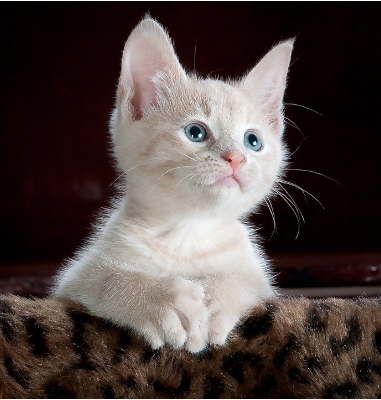
\includegraphics{gatito}

Con la opción \texttt{scale} podemos hacerla más pequeña -o más grande-.
Pero las imágenes en \LaTeX{} no están hechas para insertarse así, sino en una
figura, que es lo que nos permite alterar su alienamiento respecto al texto
y demás propiedades. La siguiente figura está insertada con este código:
\begin{figure}[H] %esta figura es para impedir que se me divida el verbatim
\begin{verbatim}
1   \begin{figure}[H]
2       \centering 
3       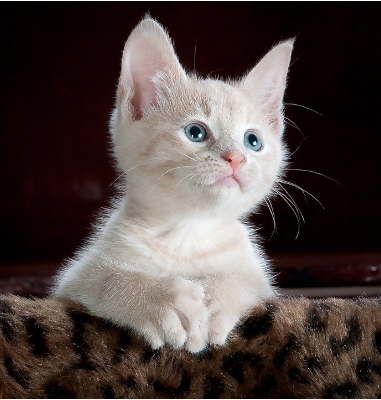
\includegraphics[width=1.0\hsize]{gatito}
4       \caption{Un gato blanco}
5       \label{fig:gatitoBlanco} 
6   \end{figure}
\end{verbatim}
\end{figure}
Vamos a analizar lo que hacen las líneas una a una:
\begin{enumerate}
   \item Crea una figura, que es un cuadro invisible para \LaTeX{}, permite
que lo que haya en ella no se divida y añadirle un título y un símbolo para
referenciarla internamente.
    \begin{itemize}
        \item la opción H (que va entre corchetes) indica a \LaTeX{} que la
        figura debe ir en el sitio en que la hemos escrito en el código, de no
        utilizar esta opción, \LaTeX{} podría decidir un lugar distinto.
    \end{itemize}
    \item Esta línea indica que la figura debe estar centrada.
    \item Esta línea es la que incluye la imagen propiamente dicha.
    \begin{itemize}
        \item La opción (entre corchetes)
            \texttt{width=1.0\textbackslash{}hsize} hace que la imagen ocupe
            el 100 \% del ancho de la página. Si cambias el número ($1,0$) por 
            ejemplo a $0,5$ ocuparía el 50 \%.
        \item Como hemos usado la orden \texttt{graphicspath} en el preámbulo.
        Podemos escribir simplemente el nombre del archivo, sin extensión.
    \end{itemize}
    \item La orden \texttt{caption} pone el título visible que tendrá la figura.
    \item La orden label crea la etiqueta interna de esta figura, y permite 
    luego referenciarla. Esta orden debe ir \textbf{después} de
        \texttt{caption}. Cada tipo de document en LaTeX tiene su prefijo, por
        ejemplo, las figuras deben ser \texttt{fig:XXX} y las tablas 
        \texttt{tab:XXX} donde \texttt{XXX} es un nombre arbitrario.
    \item Finalmente, esto termina la figura.
\end{enumerate}

El resultado es el siguiente:
% [H] inserta aquí, t al inicio de la página, b al final... hay muchas opciones
    % Usa "H" si quieres que la figura esté en el mismo orden que como la has
    % escrito, es la opción más intuitiva.
    % (ver sección donde incluyo los paquetes)
% Gracias a que hemos puesto la orden \graphicspath{{./img/}} en el preámbulo
    % de nuestro documento, ahora sólo tenemos que poner el nombre de las
    % imágenes que estén ahí.
%inicio de una figura.
\begin{figure}[H]
    % Centra la imagen
    \centering 
    % Con width=1.0\hsize hacemos que la imagen sea tan ancha como el párrafo,
    % yo lo recomiendo para que las cosas queden alineadas, salvo que por x
    % motivo quieras una imagen más pequeña, entonces cambia 1.0 por otro nº.
    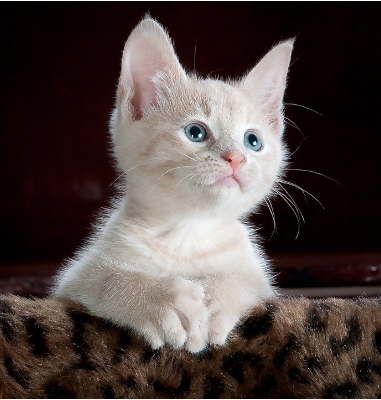
\includegraphics[width=1.0\hsize]{gatito}
    % Título de la figura que se ve
    \caption{Un gato blanco}
    % Etiqueta interna, se usa para referencias la imagen. Esta orden debe ir
    % siempre después de la caption. Cada tipo de figura tiene su formato de 
    % label, por ejemplo las figuras son fig: y las tablas tab:, respétalo o 
    % LaTeX no podrá encontrarlas para los índices.
    \label{fig:gatitoBlanco} 
\end{figure}

Al insertar un párrafo aquí podemos ver cómo se organizan las imágenes, de tal
modo que se insertan en la página necesaria. Las figuras no se dividen a sí
mismas entre páginas.

\begin{figure}[H]
    %centra la imagen (por si no quedaba claro)
    \centering
    % El número antes de hsize es un multiplicador, por ejemplo, podemos hacer
    % que ocupe un tercio de ancho
    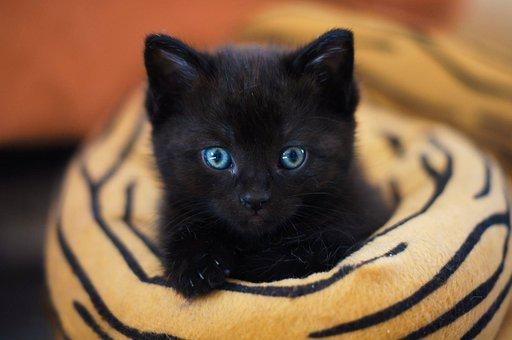
\includegraphics[width=0.3333\hsize]{gatitoNegro}
    \caption{Un gato negro} %caption que se ve
    \label{fig:gatitoNegro} %nombre interno para referenciar luego
\end{figure}

\subsubsection{Referencias cruzadas}
Una referencia cruzada es un punto en el texto en que hablamos de un elemento
del mismo, por ejemplo, si quisiéramos referenciar aquí la figura titulada
<<Un gato negro>>, podríamos ponerlo a mano en el texto: Como se puede ver
en la Figura 2: Un gato negro. Pero, ¿qué pasaría si cambiáramos ese título?
¿Y si incluyéramos una imagen antes de esta y su número cambiara? Para eso
usaremos el comando \texttt{ref}. Este comando nos permite referenciar una
figura (o cualquier objeto con una etiqueta). 

Si ahora quieres referenciar una figura en un párrafo en \LaTeX{} puedes poner
\texttt{ \textbackslash ref\{nombre de la referencia\}}. Esto insertará el 
número de la figura. Si insertamos \texttt{\textbackslash{}nameref\{nombre
de la referencia\}} aparecerá el título de la misma (la \textit{caption}).

Por ejemplo: como podemos ver en la Figura \ref{fig:gatitoNegro}:
\nameref{fig:gatitoNegro}. A continuación, vamos a insertar una tabla.

\begin{verbatim}
1   \begin{table}[H]
2       \centering
3       \begin{tabular}{|c|r|c|r|}
4           \hline
5           Concepto & Precio Unitario & Cantidad & Subtotal\\ \hline
6           Placa base & \EUR{89,99} & 1 & \EUR{89,99}\\ \hline
7           RAM 8GB DDR4 3200 MHz & \EUR{40,44} & 4 & \EUR{161,76} \\ \hline
8           \textbf{Total}&&&\textbf{\EUR{251,75}} \\ \hline
9       \end{tabular}
10  \caption{Gastos de la reparación}
11  \label{tab:gastos}
12  \end{table}
\end{verbatim}

\begin{enumerate}
\item Inicial la <<figura tabla>>, esto es equivalente a cuando incrustamos
una figura que va a contener una imagen.
\item Hace que la tabla esté centrada, aclaración: cuando la tabla es más 
grande que el tamaño del texto se alinea a la izquierda y se desborda por la
derecha.
\item Empieza la tabla en sí misma, la segunda parte \texttt{\{\{|c|r|c|r|\}\}}
indica el número de celdas (que se corresponde con el número de letras) y las 
líneas verticales (|) indican que queremos una línea entre esas dos columnas.
\item Dibuja una línea horizontal en toda la tabla
\item Es una fila de la tabla, el texto irá en la misma celda hasta que haya
un \textit{et} (\&), así se pasa de columna. Cuando se haya terminado la fila,
se deben poner dos líneas inclinadas invertidas 
(\textbackslash{}\textbackslash{}). 
\item Siguiente fila, apréciese el uso de la orden 
\texttt{\textbackslash{}EUR\{\}}. (ver: \textbf{\ref{ecuaciones}})
\item La siguiente fila.
\item La última fila, nótese que se pueden poner celdas vacías poniendo
dos \emph{et} (\&\&) Y que debe terminarse con \textbackslash{}\textbackslash{}.
\item Termina la tabla
\item Indica el título visible de la tabla.
\item Etiqueta para referencias.
\end{enumerate}
% Esto no sirve para hacer la tabla en sí misma, sino para ponerle captions y
% esas cosas. Es equivalente a \begin{figure} que no inserta una imagen, pero
% nos prepara las cosas para que se comporte como una figura, así podemos
% ponerle título y referenciarla.
\begin{table}[H]
    \centering
    % Aquí defines la tabla en sí misma, tienes que poner tantas letras como
    % columnas vaya a tener la tabla, y puedes poner líneas verticales entre
    % ellas escribiendo este símbolo entre las letras. Estas letras son los
    % especificadores de alineación. Si pones l, la columna se alinea a la
    % izquierda, si pones c, al centro, y si pones r, a la derecha.
    \begin{tabular}{|c|r|c|r|}
    % Esta orden genera una línea entre filas de la tabla.
    \hline
    % En las tablas las celdas se separan con & y las filas con \\
    % Puede haber celdas vacías, pero todas las filas deben tener las mismas
    % celdas.
    Concepto & Precio Unitario & Cantidad & Subtotal\\ \hline
    Placa base & \EUR{89,99} & 1 & \EUR{89,99}\\ \hline
    RAM 8GB DDR4 3200 MHz & \EUR{40,44} & 4 & \EUR{161,76} \\ \hline
    % Aquí podemos ver que hemos puedo celdas vacías. (dos & seguidos)
    \textbf{Total}&&&\textbf{\EUR{251,75}} \\ \hline
\end{tabular}
    % De nuevo, el título que se ve
    \caption{Gastos de la reparación}
    % La referencia interna. 
    \label{tab:gastos}
\end{table}

De nuevo, podemos referenciar el número de la tabla con \ref{tab:gastos} y su
títulos con \nameref{tab:gastos}. Nota del autor: a veces salen signos de
interrogación, no te preocupes, \LaTeX{} a veces necesita dos compilaciones para 
crear la base de datos de referencias.

Creo que ya estás listo para usar \LaTeX{}.
He incluido un fichero makefile en el directorio que debería compilar el 
archivo presente con la orden \texttt{pdflatex} dos veces.

Finalmente, incluyo un ejemplo de todas las macros de tamaños que vienen
incluidas en LaTeX base para pdflatex. Cada modificador hace que todo lo que
se escriba después de él se vea afectado. Por esto, debe volverse al tamaño
normal.

\tiny{Ejemplo de texto tiny}\normalsize

\scriptsize{Ejemplo de texto scriptsize}\normalsize

\footnotesize{Ejemplo de texto footnotesize}\normalsize

\small{Ejemplo de texto small}\normalsize

\normalsize{Ejemplo de texto normalsize}\normalsize

\large{Ejemplo de texto large}\normalsize

\Large{Ejemplo de texto Large}\normalsize

\LARGE{Ejemplo de texto LARGE}\normalsize

\huge{Ejemplo de texto huge}\normalsize

\Huge{Ejemplo de texto Huge}\normalsize

\section{Licencias y agradecimiento}

Todas las páginas citadas son de sus respectivos creadores, yo sólo me limito
a recopilar sus soluciones o información en un mismo documento. Todas las
imágenes utilizadas son de licencia libre, ver:
\href{https://pixabay.com/service/faq/}{FAQ de Pixabay}

\end{document}
